\chapter{Simulation results}
\label{chap-simulation}

This chapter describes numerical simulations carried out to demonstrate and evaluate the disturbance models and observer designs described in Chapter \ref{chap-methods}. Section \ref{sim-RODDs} describes simulated examples of different RODDs. Section \ref{sim-obs-lin} describes experiments to evaluate the two observers in estimating the states of two simulated systems, a single-input single-output (SISO) linear system with one RODD step disturbance, followed by a 2-input, 2-output linear system with two RODD step disturbances. Section \ref{sim-ore-SISO} describes an experiment to evaluate the observers on the simulated grinding circuit model with one output variable and a step disturbance in the ore feed mix. Section \ref{sim-ore-MIMO} describes an experiment to evaluate the observers in a multi-variable feedback control scenario with the simulated grinding circuit model.


\section{Generating RODD disturbances} \label{sim-RODDs}

RODDs are easy to generate by numerical simulation.  Plot (a) in Figure \ref{fig:rodd-sim-plots} shows a random shock sequence (\ref{eq:wpk1}) of length 1000 samples generated using a pseudo random number generator. Plots (b), (c), and (d) show RODD step, ramp and exponential change disturbances generated with this random shock sequence using the RODD models in (\ref{eq:RODD-step}), (\ref{eq:RODD-ramp}), and (\ref{eq:RODD-exp}). 

\begin{figure}[htp]
	\centering
	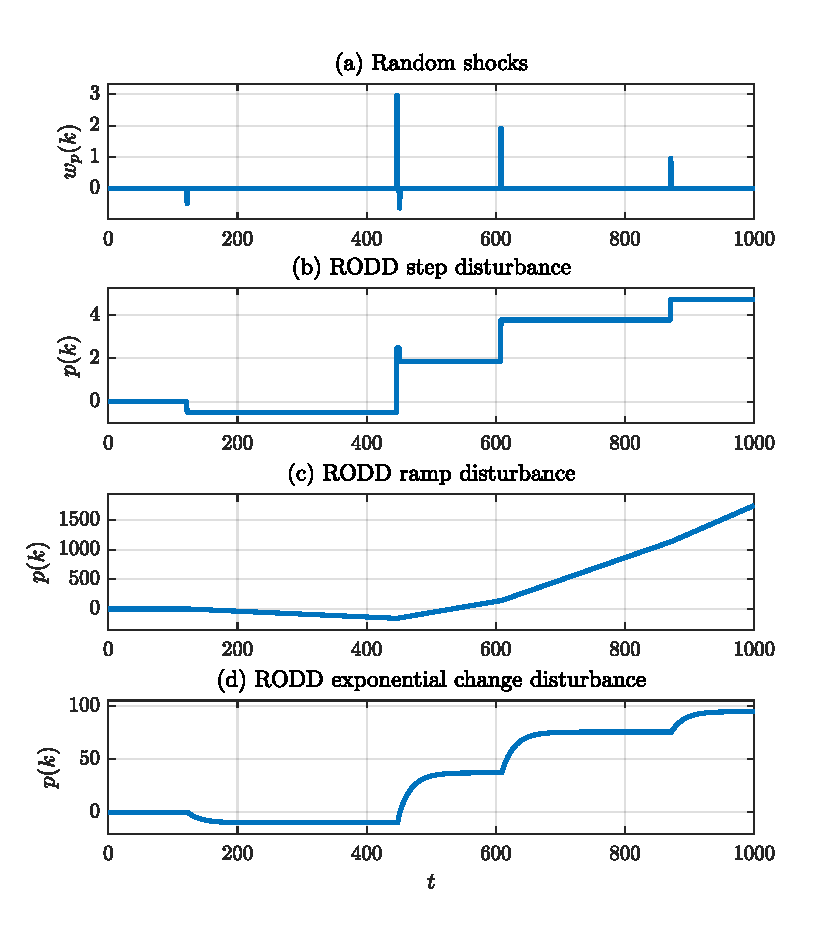
\includegraphics[width=13.5cm]{images/rodd_sim_plots.pdf}
	\caption{Examples of RODDs}
	\label{fig:rodd-sim-plots}
\end{figure}

\begin{figure}[htp]
	\centering
	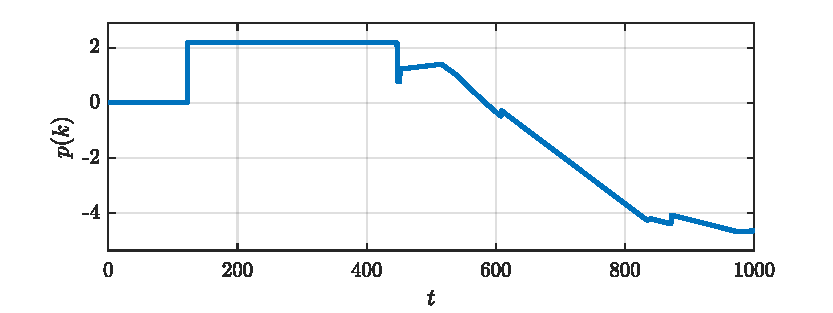
\includegraphics[width=13.5cm]{images/rodd_sim_plot2.pdf}
	\caption{RODD with steps and ramps}
	\label{fig:rodd-sim-plot2}
\end{figure}


\section{Estimating RODD disturbances} \label{sim-obs-lin}

\subsection{SISO linear system} \label{sim-obs-lin-1}

To demonstrate state estimation in the presence of RODDs, a single RODD was simulated at the input to a process represented by a discrete-time linear model, as shown in the functional diagram in \ref{fig:sim-sys-diag-siso}. In addition to the input disturbance, the process model has an input variable, $u(k)$, and a measured output variable, $y(k)$. A random noise $v(k)$ with zero mean and standard deviation $\sigma_M$ is added to the output of the process to represent measurement errors. At each sample time, the input and measured output are passed to an observer which calculates estimates of the process states at the next sample time, $\hat{x}(k+1)$.

\begin{figure}[htp]
	\centering
	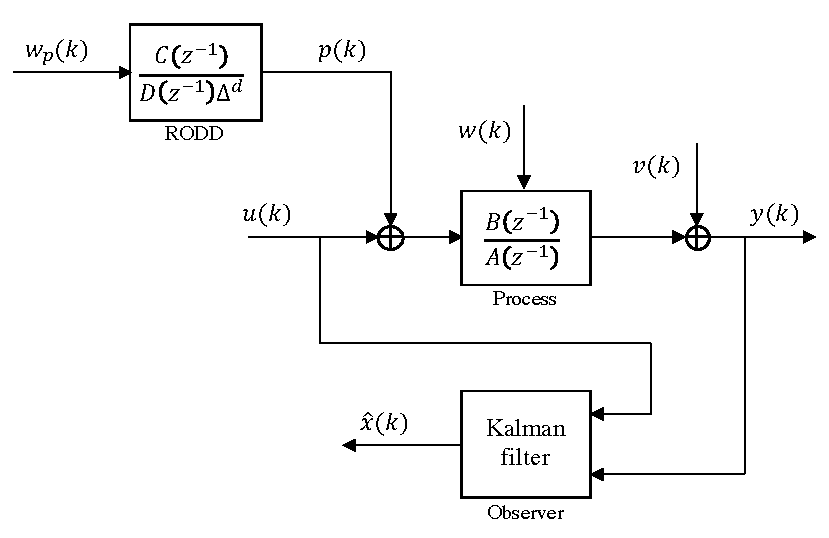
\includegraphics[width=11.5cm]{images/sim-sys-diag-siso.pdf}
	\caption{Functional diagram of the simulated SISO system with observer}
	\label{fig:sim-sys-diag-siso}
\end{figure}

For the purposes of this experiment, the linear model used to represent the process was a first order, stable system,
\begin{equation}
	\frac{B(z^{-1})}{A(z^{-1})} = \frac{0.3z^{-1}}{1-0.7z^{-1}}
\end{equation}
with a sampling period of $T=0.5$.

The RODD was a step disturbance defined by
\begin{equation}
	\frac{C(z^{-1})}{D(z^{-1})} = \frac{1}{1-z^{-1}}
\end{equation}
with $w_p(k)$ defined by (\ref{eq:wpik2}) and $\epsilon=0.01$, $\sigma_{w_p}=0.01$, and $b=100$.

The state-space representation used to simulate the augmented system was
\begin{equation} \label{eq:sim-sys-siso-ss-aug}
	\begin{split}
	\mathbf{x}_{a}(k+1) & =\left[\begin{array}{cc}
		0.7 & 1 \\
		0 & 1
	\end{array}\right] \mathbf{x}_{a}(k)+\left[\begin{array}{l}
		1 \\
		0
	\end{array}\right] u(k) + \mathbf{w}_{a}(k) \\
	y(k) & =\left[\begin{array}{cc}
	0.3 & 0
\end{array}\right] \mathbf{x}_{a}(k) + v(k)
\end{split}
\end{equation}
where
\begin{equation} \label{eq:sim-sys-siso-ss-aug2}
		\mathbf{x}_{a}(k) = \left[\begin{array}{l}
			x_{a,1}(k) \\
			x_{a,2}(k)
		\end{array}\right] = \left[\begin{array}{l}
		x_{1}(k) \\
		p(k)
	\end{array}\right], \mathbf{w}_{a}(k) = \left[\begin{array}{l}
	w_1(k) \\
	w_{p}(k)
\end{array}\right] .
\end{equation}

Note that with this choice of model, the unmeasured disturbance $p(k)$ corresponds exactly to the second model state, $x_{a,2}(k)$.

Figure \ref{fig:sim-sys-siso-ioplot} shows a set of input-output data generated by simulating this system for a duration of 300 time units to generate 600 data samples. The lower of the two plots shows the input signals, $u(k)$ and $p(k)$. From this it can be seen that 7 random shocks occurred of various magnitudes and that in between these, the value of $p(k)$ is a random walk due to the persistent component of the RODD disturbance (i.e. in the absence of the infrequent random shocks). In addition, a step change in $u(k)$ of magnitude 1 occurred at time $t=5$. The upper plot shows the simulated output measurements. The standard deviation of the measurement noise, $\sigma_M$, was $0.1$. No input disturbances other than $w_p(k)$ were simulated (i.e. $\mathbf{w}(k)=w_1(k)=0$). 
\begin{figure}[htp]
	\centering
	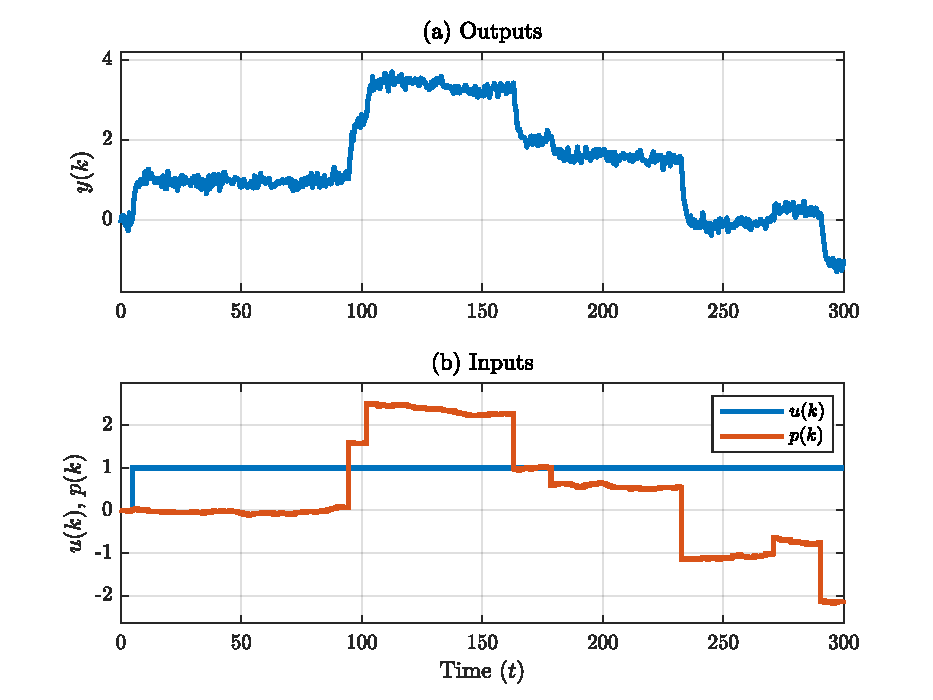
\includegraphics[width=14cm]{images/sim_sys_1_3_ioplot.pdf}
	\caption{Simulation of linear system with a RODD input disturbance}
	\label{fig:sim-sys-siso-ioplot}
\end{figure}

A standard Kalman filter was used to develop performance baselines with which to evaluate the sub-optimal multi-model observers. The question of how to set the gain of a Kalman filter when there is a RODD affecting the system is open to interpretation. One naive approach is to tune the Kalman filter using the variance of the persistent component of the disturbance, $\sigma_{w_p}^2$, which is known in these simulated experiments. In this case, the Kalman filter, which is labelled `KF1', has a state disturbance covariance matrix
\begin{equation} \label{eq:sim-sys-siso-KF1-Q}
	\begin{aligned}
		\mathbf{Q}_{\text{KF1}}=\mathbf{Q}_0=\begin{bmatrix}
			\sigma_{x_1}^2 & 0 \\
			0 &  \sigma_{w_p}^2 \\
		\end{bmatrix}=\begin{bmatrix}
		0.01^2 & 0 \\
		0 & 0.01^2 \\
	\end{bmatrix}
	\end{aligned},
\end{equation}
where $\sigma_{x_1}^2$ is the variance of the estimates of the process model state, $x_1$. The value $\sigma_{x_1}=0.01$ was chosen because the simulated process model is identical to the model used by the observers and no additional disturbances are applied to the process model states during simulations (i.e. $w_1(k)$ in (\ref{eq:sim-sys-siso-ss-aug2}) is 0).

However, this leads to a filter with a slow response to the shocks. A second option is to tune the Kalman filter to the variance of the random shocks, $b^2\sigma_{w_p}^2$.  In this case, the Kalman filter, labelled `KF2', has a state disturbance covariance matrix
\begin{equation} \label{eq:sim-sys-siso-KF2-Q}
	\begin{aligned}
		\mathbf{Q}_{\text{KF2}}=\mathbf{Q}_1=\begin{bmatrix}
			\sigma_{x_1}^2 & 0 \\
			0 & b^2\sigma_{w_p}^2 \\
		\end{bmatrix}=\begin{bmatrix}
			0.01^2 & 0 \\
			0 & 1^2 \\
		\end{bmatrix}.
	\end{aligned}
\end{equation}

The problem with this filter is that it is very sensitive to the measurement noise, $v(k)$. As explained in \cite{robertson_detection_1995}, a trade off is needed. One approach to making this trade-off is to minimize the average estimation errors over a suitably long set of input-output data. An approximate solution to this problem was found by running multiple evaluations of the Kalman filter with different tunings until a minimum RMSE was found. Figure \ref{fig:sim-sys-siso-KF3-tuning} shows the results of these evaluations, from which it can be seen that the lowest RMSEs for both estimates occur when the variance parameter $\sigma_{w_p}^2$ is close to $0.01$. Using this result, a third Kalman filter labelled `KF3' was designed with the state disturbance covariance matrix 
\begin{equation} \label{eq:sim-sys-siso-KF3-Q}
	\begin{aligned}
		\mathbf{Q}_{\text{KF3}}=\mathbf{Q}_{\text{opt}}=\begin{bmatrix}
			\sigma_{x_1}^2 & 0 \\
			0 & \sigma_{w_p,\text{opt}}^2 \\
		\end{bmatrix}=\begin{bmatrix}
			0.01^2 & 0 \\
			0 & 0.1^2 \\
		\end{bmatrix}.
	\end{aligned}
\end{equation}

\begin{figure}[htp]
	\centering
	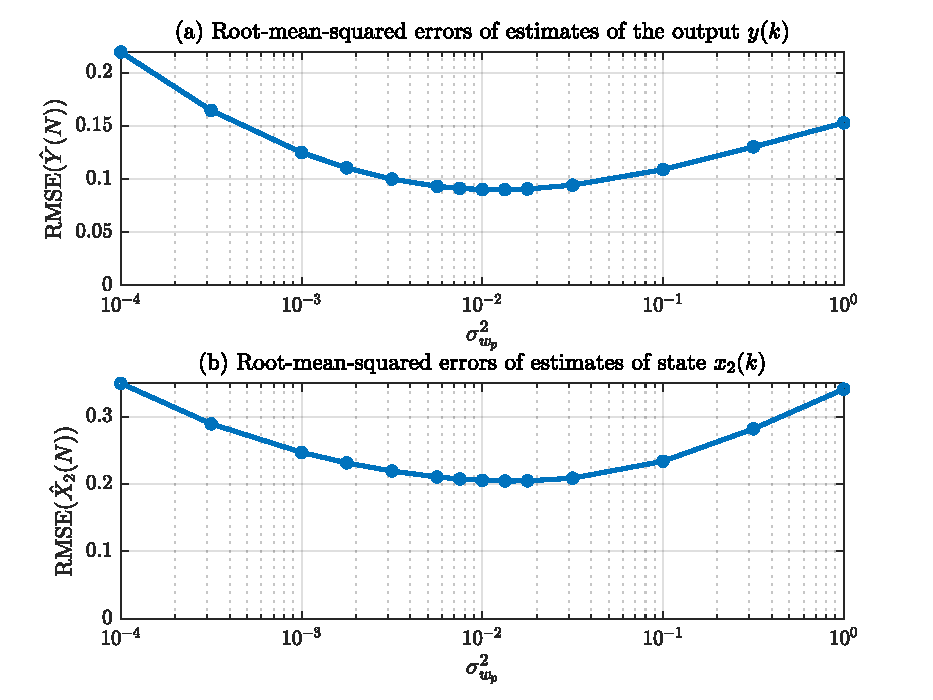
\includegraphics[width=14cm]{images/rod_obs_sim1_plot_KF3_tuning.pdf}
	\caption{Tuning of a Kalman filter to minimise estimation errors}
	\label{fig:sim-sys-siso-KF3-tuning}
\end{figure}

Figure \ref{fig:sim-sys-siso-KF123-est} shows the state and output estimates of each of the three Kalman filters described above on the simulated input-output data. As expected, the response of KF1 to the infrequent step disturbances is noticeably slower than that of the other two. The response of KF2 is fast, but it is sensitive to the measurement noise. KF3 is a compromise between the two—relatively fast response to the infrequent step changes, while having less sensitivity to the measurement noise.
\begin{figure}[htp]
	\centering
	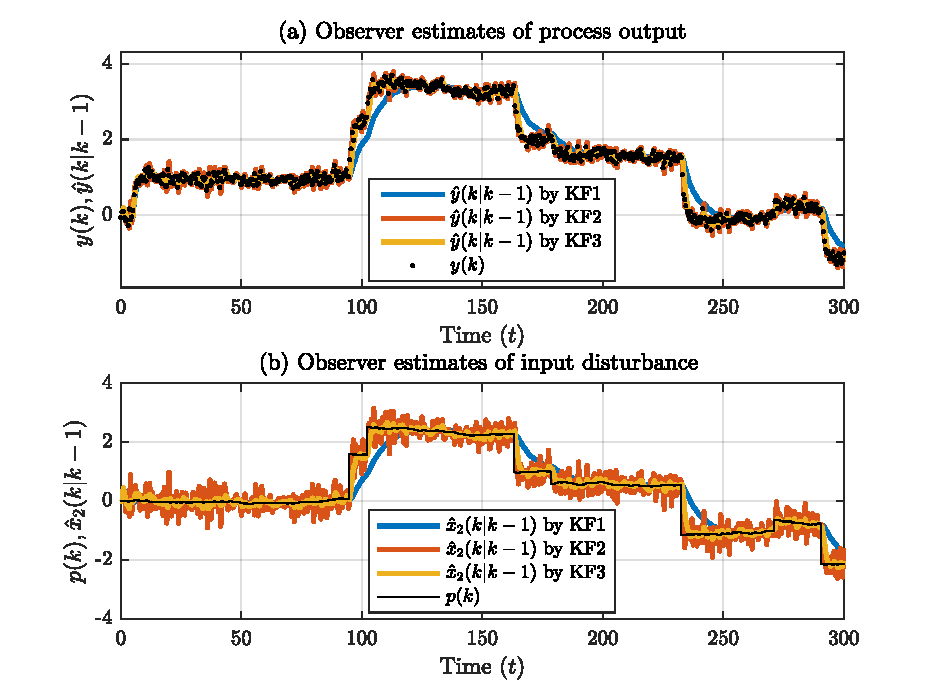
\includegraphics[width=14cm]{images/sim_sys_1_3_est.pdf}
	\caption{Kalman filter estimates}
	\label{fig:sim-sys-siso-KF123-est}
\end{figure}

The upper plot in Figure \ref{fig:sim-sys-siso-KF123-cumerr} shows the errors in the output estimates of each Kalman filter when compared to the true process outputs (ignoring measurement noise). The lower plot shows the cumulative sum of the squared errors. This clearly shows the differences in performance between the three filters. The estimation errors of KF1 are small when the system is in steady-state but increase dramatically after each step disturbance. The magnitude of the errors of KF2 is higher during steady-state periods but remains roughly constant throughout the simulation. KF3 achieves the lowest overall cumulative sum-of-squared-errors by the end of the simulation.
\begin{figure}[htp]
	\centering
	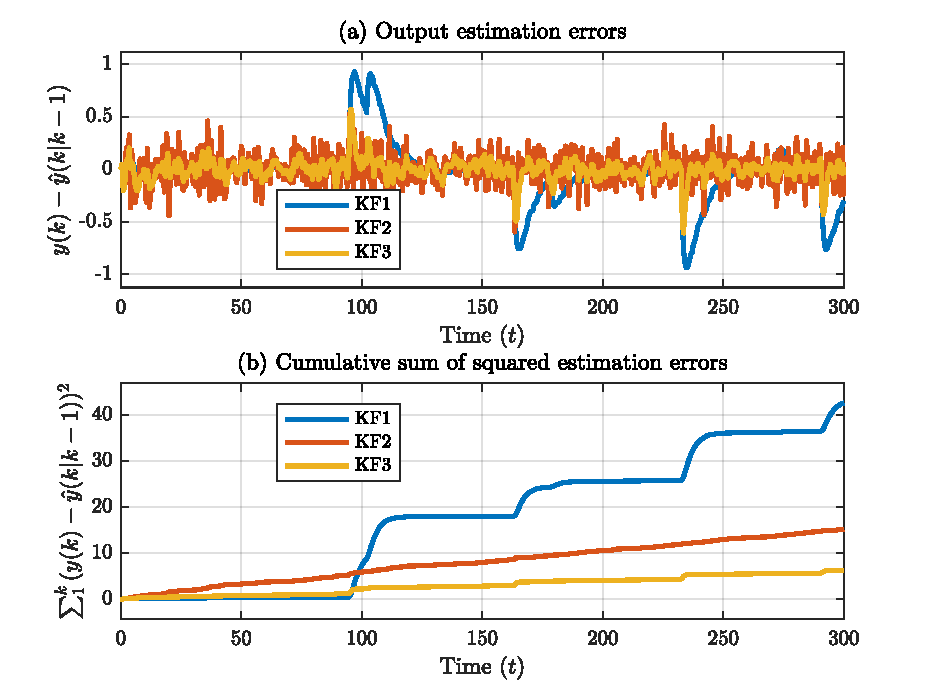
\includegraphics[width=14cm]{images/sim_sys_1_3_y1_err.pdf}
	\caption{Cumulative errors of Kalman filter estimates}
	\label{fig:sim-sys-siso-KF123-cumerr}
\end{figure}

The two sub-optimal multi-model observer algorithms were also tested on data from this system. The best choice of values for these parameters was determined by running multiple simulations with different parameter values and evaluating the observer performance. 

The sequence fusion algorithm proposed by \cite{robertson_method_1998} has three parameters which must be specified, $n_f$, $n_d$, and $n_m$, as described in Section \ref{subsec-fusion}. Candidate values for these parameters were found by considering every combination of $n_f$, $n_m$, and $n_d$ satisfying

\begin{equation} \label{eq:sim-sys-siso-MKF-SF-param-values}
	\begin{aligned}
		\frac{n_f}{n_d} \in \left\{3, 5, 10, 15, 20\right\},  \\
		n_m \in \left\{1, 2, 3\right\},  \\
		n_d \in \left\{1, 2, 3, 5, 10\right\}.  \\
	\end{aligned}
\end{equation}

Note that $\frac{n_f}{n_d}$ represents the number of detection intervals within the fusion horizon and is always a whole number. Combinations where rejected when the number of hypotheses, $n_h$, was greater than 500 and when the total probability modelled, $\beta$ (\ref{eq:p_gamma}), was less than 0.85. Each remaining combination was then evaluated by calculating the RMSE of the output estimates of the observer on 5000 samples from the simulated system (Figure \ref{fig:sim-sys-diag-siso}). Table \ref{tb:obs-sim1-popt-SF} shows the best 10 combinations of parameter values (those with the lowest RMSE).

\begin{table}[hb]
	\begin{center}
		\caption{Multi-model observer parameter search results – MMKF-SF.} \label{tb:obs-sim1-popt-SF}
		% See: https://texblog.org/2019/06/03/control-the-width-of-table-columns-tabular-in-latex/
		\begin{tabular}{p{0.05\textwidth}>{\centering\arraybackslash}p{0.07\textwidth}>{\centering\arraybackslash}p{0.07\textwidth}>{\centering\arraybackslash}p{0.07\textwidth}>{\centering\arraybackslash}p{0.07\textwidth}>{\centering\arraybackslash}p{0.24\textwidth}}
			$n_f$ & $n_m$ & $n_d$ & $n_h$ & $\beta$ & $\text{RMSE}(\hat{Y}(N),Y(N))$   \\
			\hline
% Results with seed = 2.
			10 &   3 &   1 & 176 & 1.0000 & 0.1115 \\
			10 &   2 &   1 &  56 & 0.9999 & 0.1115 \\
			10 &   1 &   1 &  11 & 0.9957 & 0.1115 \\
			10 &   3 &   2 &  26 & 1.0000 & 0.1137 \\
			10 &   2 &   2 &  16 & 0.9999 & 0.1137 \\
			10 &   1 &   2 &   6 & 0.9962 & 0.1137 \\
			15 &   3 &   5 &   8 & 1.0000 & 0.1157 \\
			15 &   2 &   5 &   7 & 0.9999 & 0.1157 \\
			15 &   1 &   5 &   4 & 0.9930 & 0.1157 \\
			15 &   3 &   3 &  26 & 1.0000 & 0.1165 \\
% seed = 0
%			15 &   1 &   5 &   4 & 0.9930 & 0.1113 \\
%			15 &   3 &   5 &   8 & 1.0000 & 0.1113 \\
%			15 &   2 &   5 &   7 & 0.9999 & 0.1113 \\
%			10 &   1 &   1 &  11 & 0.9957 & 0.1126 \\
%			10 &   2 &   1 &  56 & 0.9999 & 0.1126 \\
%			10 &   3 &   1 & 176 & 1.0000 & 0.1126 \\
%			15 &   1 &   3 &   6 & 0.9917 & 0.1139 \\
%			15 &   2 &   3 &  16 & 0.9997 & 0.1139 \\
%			15 &   3 &   3 &  26 & 1.0000 & 0.1139 \\
%			15 &   1 &   1 &  16 & 0.9904 & 0.1145 \\
			\hline
		\end{tabular}
	\end{center}
\end{table}

A fusion horizon of $n_f=10$ sample periods produced the best results of those evaluated. For this horizon length, the lowest errors were produced when the length of the detection interval was one sample period ($n_d=1$) . Increasing the maximum possible number of shocks during the fusion horizon ($n_m$) has very little additional benefit but significantly impacts the number of hypotheses to be modelled ($n_h$), and thus, the number of filters needed. Note that the differences in the RMSEs of the best 10 combinations are not large. The values chosen for the multi-model observer with sequence fusion used in the simulations in this section, which is labelled `MMKF-SF1', were $n_f=10$, $n_{min}=1$, and $n_d=1$.

The sequence pruning algorithm proposed by \cite{andersson_adaptive_1985} has only two parameters to be specified, $n_h$, and $n_{min}$, as described in Section \ref{subsec-pruning}. Candidate values for these parameters were found by considering every combination satisfying

\begin{equation} \label{eq:sim-sys-siso-MKF-SP-param-values}
	\begin{aligned}
		n_h \in \left\{3, 4, 5, 7, 10, 14, 19, 25\right\},  \\
			n_{min} \in \left\{1, 2, 3, 4, 5, 6, 7, 9, 12, 16, 21\right\}.  \\
		\end{aligned}
	\end{equation}

Combinations where rejected when $n_h - n_{min} < 1$, or in other words, when the minimum life $n_{min}$ was greater than or equal to the number of hypotheses, $n_h$. This is a necessary condition because there must be enough filters to simulate the hypotheses until they are pruned. Each remaining combination was then evaluated by calculating the RMSE of the output estimates of the observer on the same 5000 samples used in the tuning of the MMKF-SF1 observer, as described above. Table \ref{tb:obs-sim1-popt-SP} shows the 10 combinations of parameter values with the lowest RMSE.

\begin{table}[hb]
	\begin{center}
		\caption{Multi-model observer parameter search results – MMKF-SP.} \label{tb:obs-sim1-popt-SP}
		% See: https://texblog.org/2019/06/03/control-the-width-of-table-columns-tabular-in-latex/
		\begin{tabular}{p{0.05\textwidth}>{\centering\arraybackslash}p{0.07\textwidth}>{\centering\arraybackslash}p{0.24\textwidth}}
			$n_h$ & $n_\text{min}$ & $\text{RMSE}(\hat{Y}_i(N),Y_i(N))$  \\
			\hline
			% seed = 0
%			  7 &   3 & 0.0569  \\
%			10 &   8 & 0.0570  \\
%			14 &  12 & 0.0570  \\
%			25 &  22 & 0.0570  \\
%			10 &   3 & 0.0570  \\
%			20 &  17 & 0.0570  \\
%			14 &   3 & 0.0570  \\
%			14 &   4 & 0.0570  \\
%			14 &   8 & 0.0571  \\
%			50 &  44 & 0.0571  \\
				  7 &   4 & 0.0608  \\
				10 &   6 & 0.0609  \\
				10 &   7 & 0.0609  \\
				10 &   5 & 0.0609  \\
				19 &  16 & 0.0609  \\
				25 &  21 & 0.0609  \\
				7 &   3 & 0.0609  \\
				10 &   4 & 0.0609  \\
				14 &   5 & 0.0609  \\
				14 &   6 & 0.0609  \\
			\hline
		\end{tabular}
	\end{center}
\end{table}

Again, the differences between the RMSEs of the best 10 combinations are very small, indicating that the precise choice of parameters is not important in this case. The combination $n_h=7$ and $n_{min}=4$ produces the lowest RMSE of those evaluated, therefore these values were chosen for the observer, which is labelled `MMKF-SP1'. It may also be noted that the best RMSEs of this observer are significantly lower than those of the best sequence fusion observer in Table \ref{tb:obs-sim1-popt-SF}. The parameters for all the observers used in the simulations in this section are summarised in Table \ref{tb:obs-params}.

\begin{table}[hb]
	\begin{center}
		\caption{Observers and parameters – simulation {\#1}.} \label{tb:obs-params}
		% See: https://texblog.org/2019/06/03/control-the-width-of-table-columns-tabular-in-latex/
		\begin{tabular}{p{0.15\textwidth}>{\centering\arraybackslash}p{0.09\textwidth}>{\centering\arraybackslash}p{0.09\textwidth}>{\centering\arraybackslash}p{0.09\textwidth}>{\centering\arraybackslash}p{0.16\textwidth}>{\centering\arraybackslash}p{0.16\textwidth}}
			& KF1 & KF2 & KF3 & MMKF-SF1 & MMKF-SP1 \\
			\hline
			Type & Kalman filter & Kalman filter & Kalman filter & Multi-model Kalman filter & Multi-model Kalman filter \\
			Sub-optimal algorithm & - & - & - & Sequence fusion & Sequence pruning \\
			\hline
			Parameters &  &  &  & &  \\
			$\mathbf{Q}$ & $\mathbf{Q}_0$ & $\mathbf{Q}_1$ & $\mathbf{Q}_{opt}$ & $\{\mathbf{Q}_0,\mathbf{Q}_1\}$ & $\{\mathbf{Q}_0,\mathbf{Q}_1\}$ \\
			$R$ & $0.1^2$ & $0.1^2$ & $0.1^2$ & $0.1^2$ & $0.1^2$ \\
			$\mathbf{P}(0)$ & $\mathbf{P}_0$ & $\mathbf{P}_0$ & $\mathbf{P}_0$ & $\mathbf{P}_0$ & $\mathbf{P}_0$ \\
			No. of filters & 1 & 1 & 1 & 11 & 7 \\
			$n_f$ & - & - & - & 10 & - \\
			$n_m$ & - & - & - & 1 & - \\
			$n_d$ & - & - & - & 1 & - \\
			$n_{min}$ & - & - & - & - & 4 \\
			$\epsilon$ & - & - & - & 0.01 & 0.01 \\
			$\sigma_{w_p}$ & - & - & - & 1 & 1 \\
			$b$ & - & - & - & 100 & 100 \\
			\hline
		\end{tabular}
	\end{center}
\end{table}

\begin{itemize}
	\item Figure showing two sets of sequences considered.
	\item Sequence fusion observer simulation results - state and output estimates vs. true values.
	\item Analysis of internal workings to explain apparent problems with responding to shocks.
	\item Waterfall plots of observer internal variables—p(Gamma|Y), K, trace(P).
	\item Tuning of sequence pruning (Eriksson and Isaksson) sub-optimal observer.
	\item Summary table of parameter optimization results.
	\item Sequence pruning observer simulation results - state and output estimates vs. true values.
	\item Summary table of all multi-model observer parameters.
	\item Comparison of multi-model observer simulation results—hidden state and output estimates plot.
	\item Comparison of multi-model observer simulation results—cumulative estimation errors.
	\item Comparison of observer simulation results—MSE bar chart summary.
	\item Summary table comparing performance metrics for all three observers (KF3, MKF-SF, MKF-SP) - metrics: MSE, MSE-transitions, MSE-steady-state, variance-steady-state, MSD-steady-state.
	\item Discussion: Compare and contrast -> sequence pruning approach (Eriksson and Isaksson) works better.
	\item Conclude on pros, cons of each algorithm and decision to use sequence pruning for grinding simulation experiments.
\end{itemize}

\begin{figure}[htp]
	\centering
	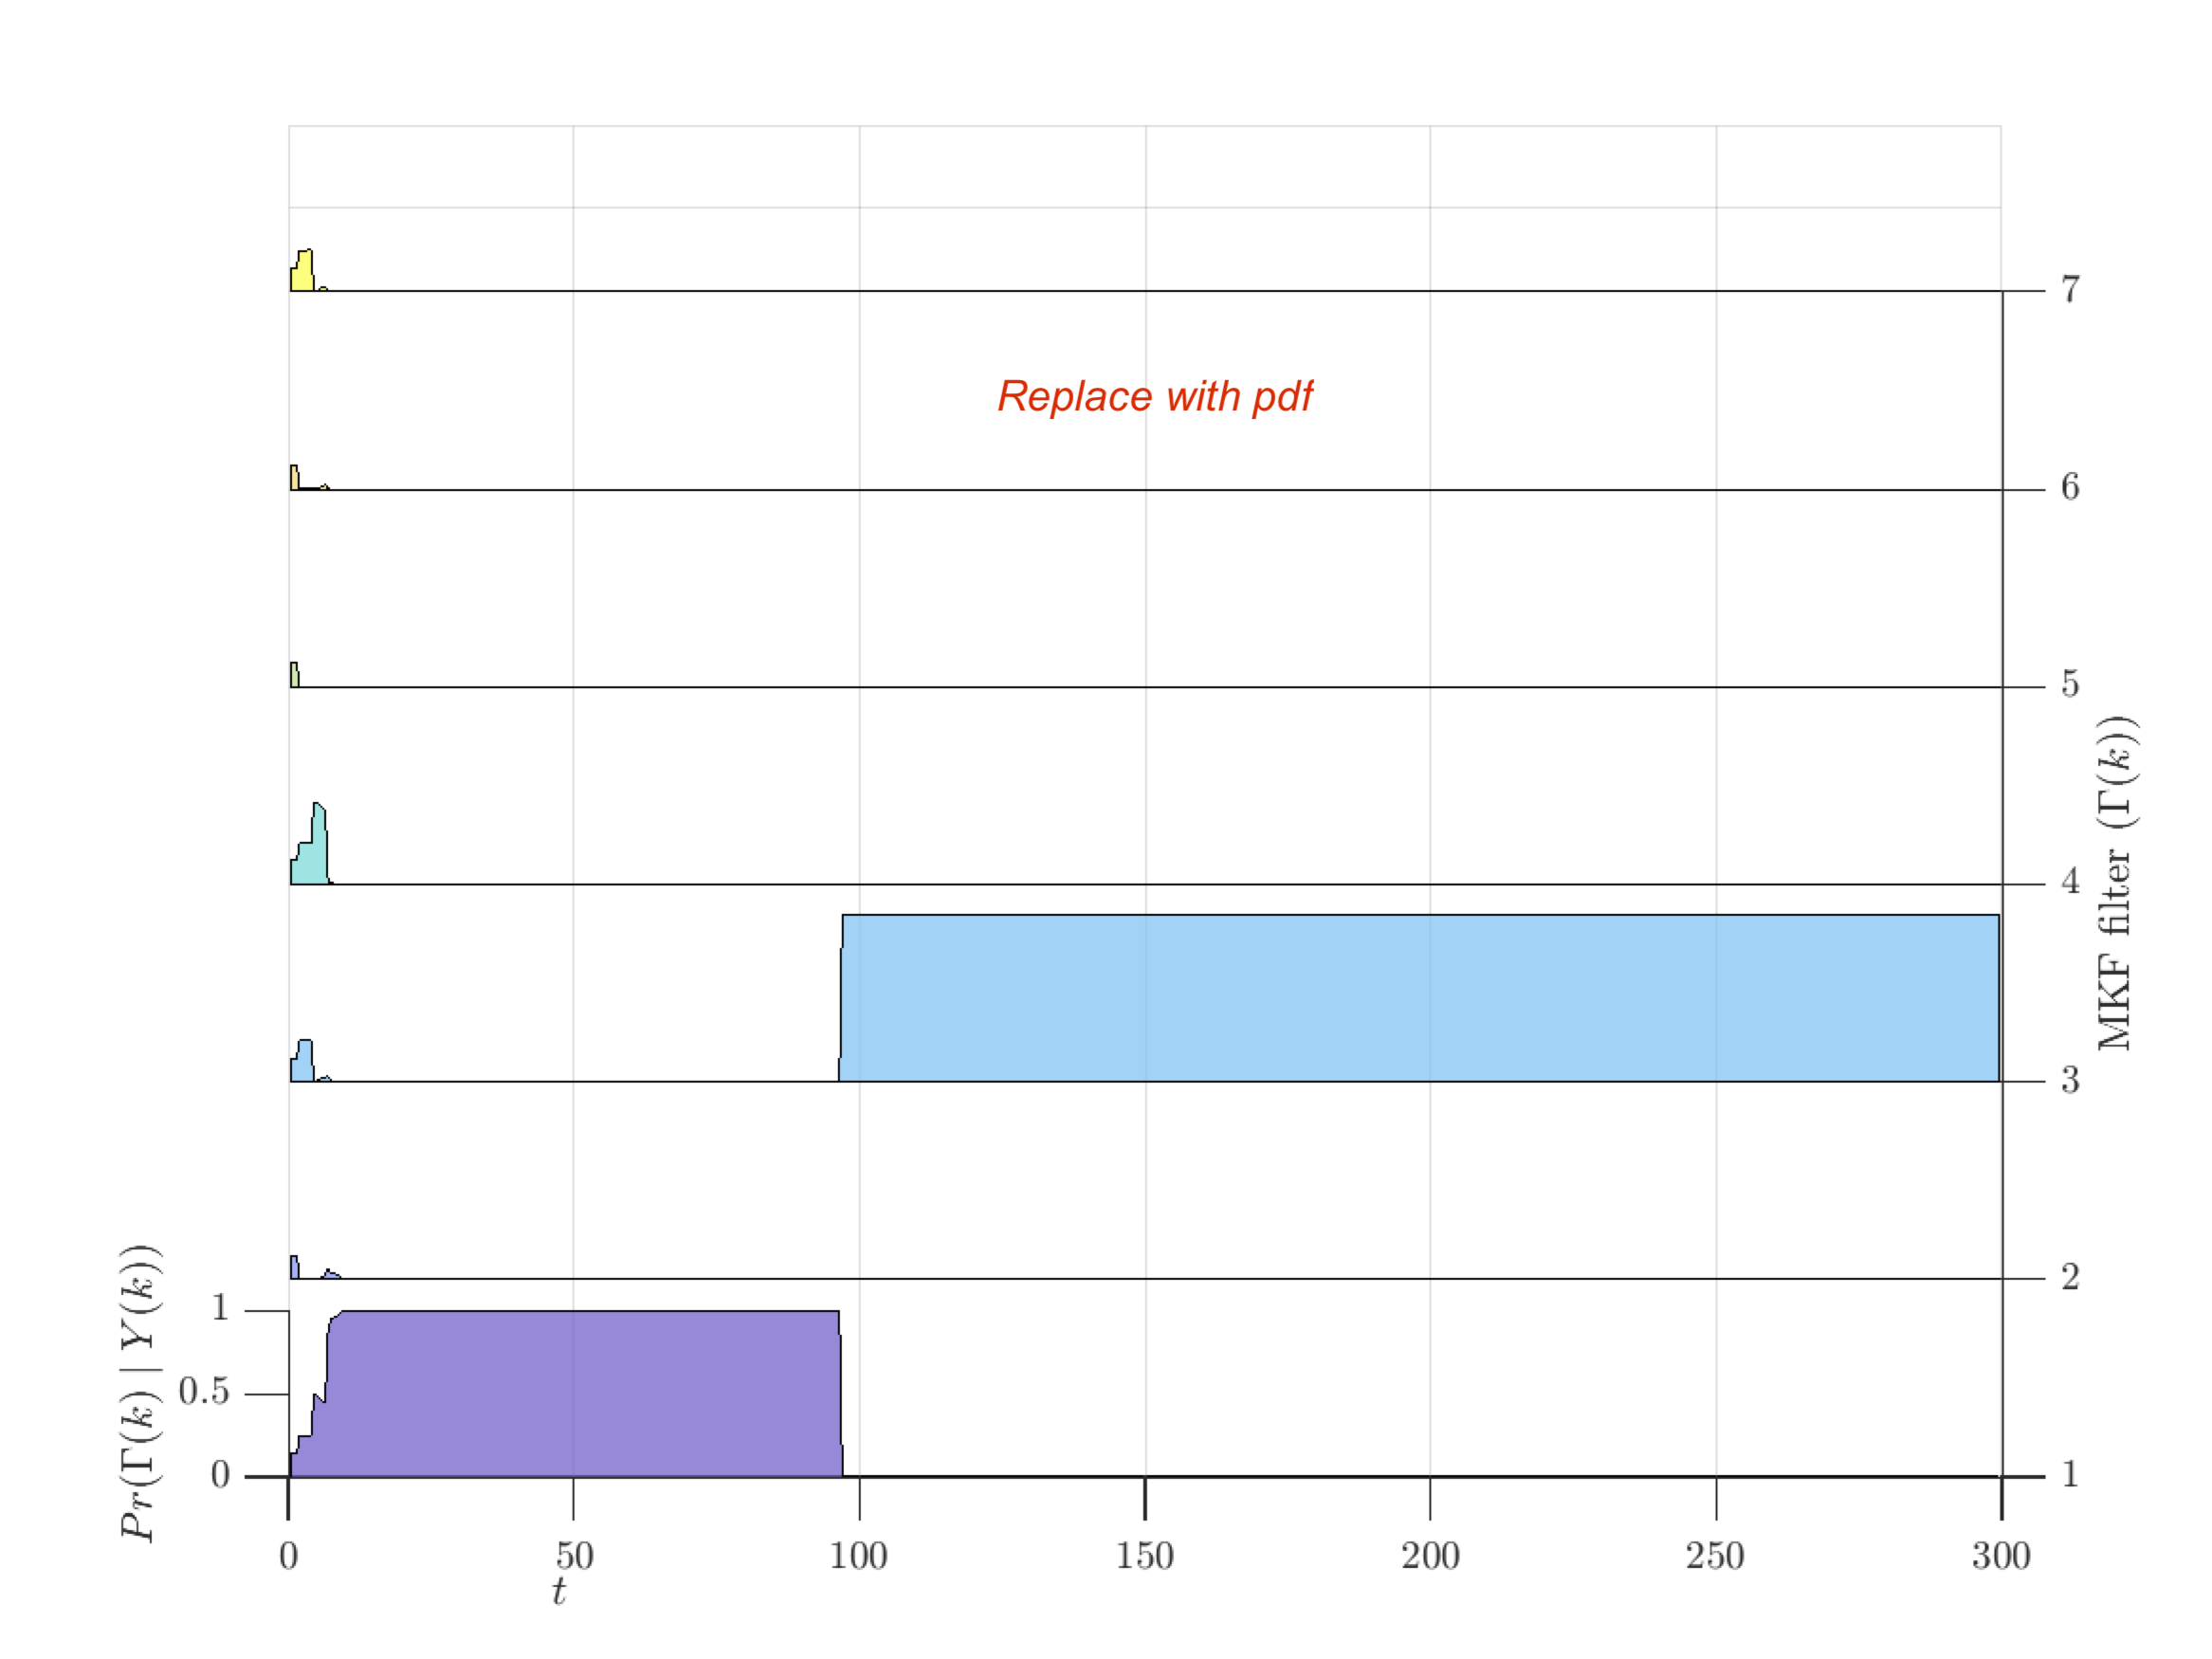
\includegraphics[width=15cm]{images/rod-obs-sim-1-4-wfplot-DRAFT.png}
	\caption{Evolution of conditional probabilities with sequence fusion}
	\label{fig:rod-obs-sim-1-4-wfplot}
\end{figure}

\begin{figure}[htp]
	\centering
	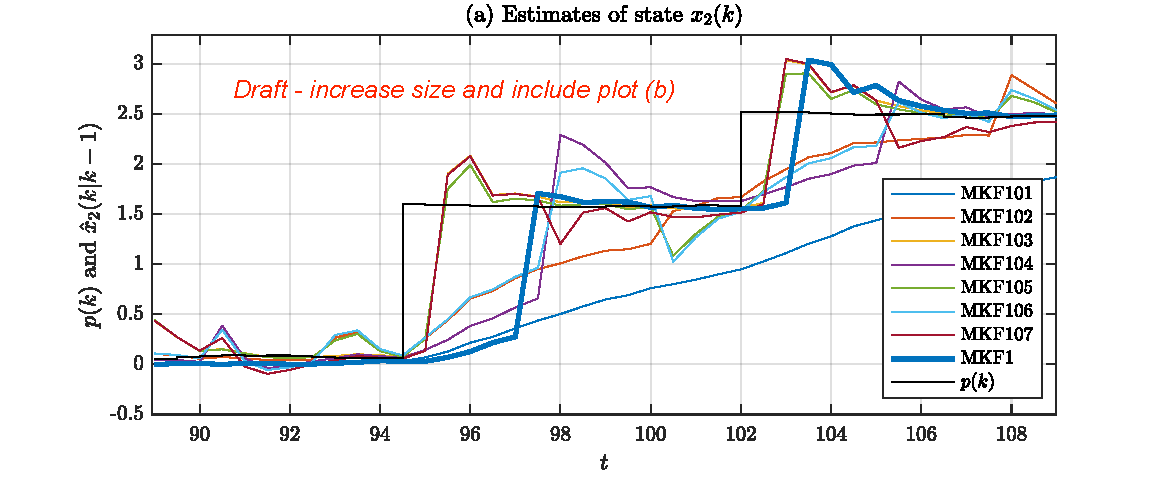
\includegraphics[width=14cm]{images/rod-obs-sim-1-4-est-MKF-SF-plot-DRAFT.pdf}
	\caption{Filter estimates of sequence fusion observer during step disturbances}
	\label{fig:rod-obs-sim-1-4-est-MKF-SF-plot-DRAFT}
\end{figure}

\begin{figure}[htp]
	\centering
	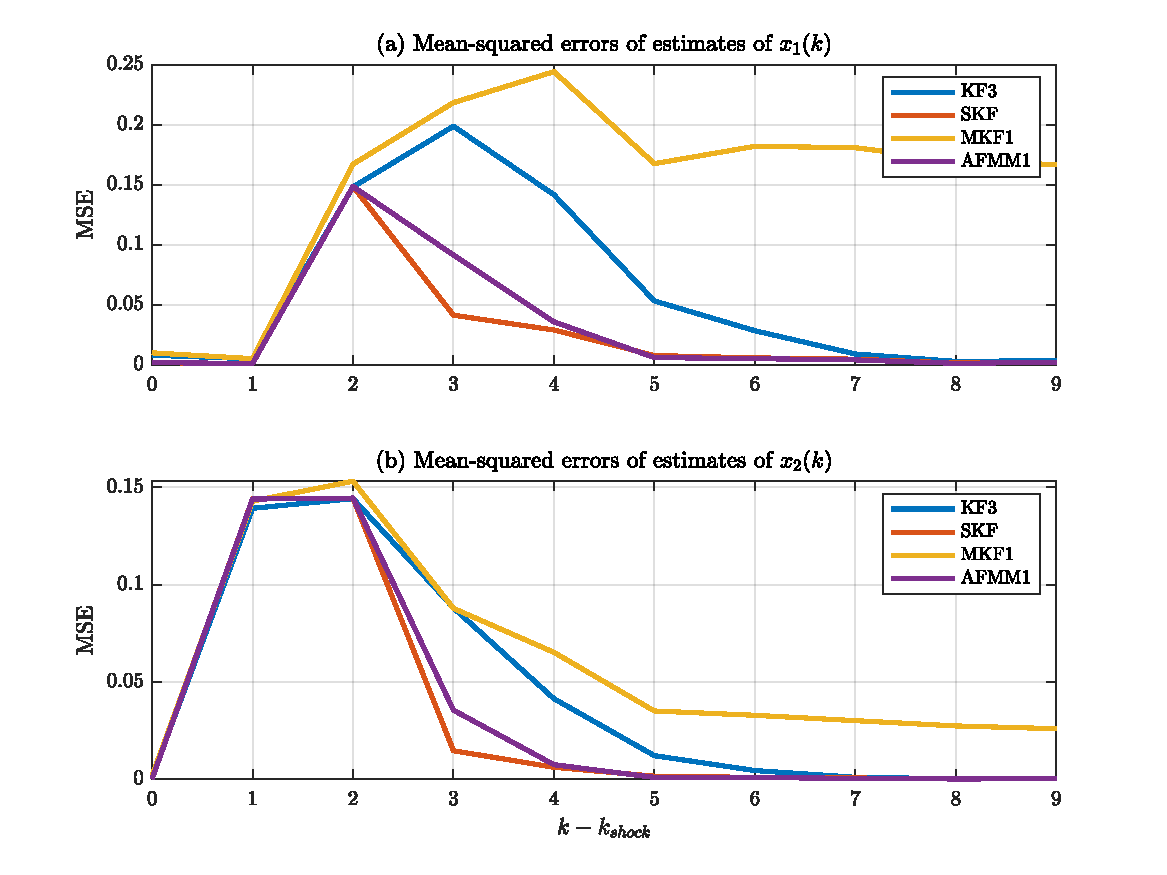
\includegraphics[width=14cm]{images/rod_obs_sim2_7_mse_ashocks.pdf}
	\caption{Average errors of observer estimates after shock disturbances}
	\label{fig:rod_obs_sim2_7_mse_ashocks}
\end{figure}

\begin{figure}[htp]
	\centering
	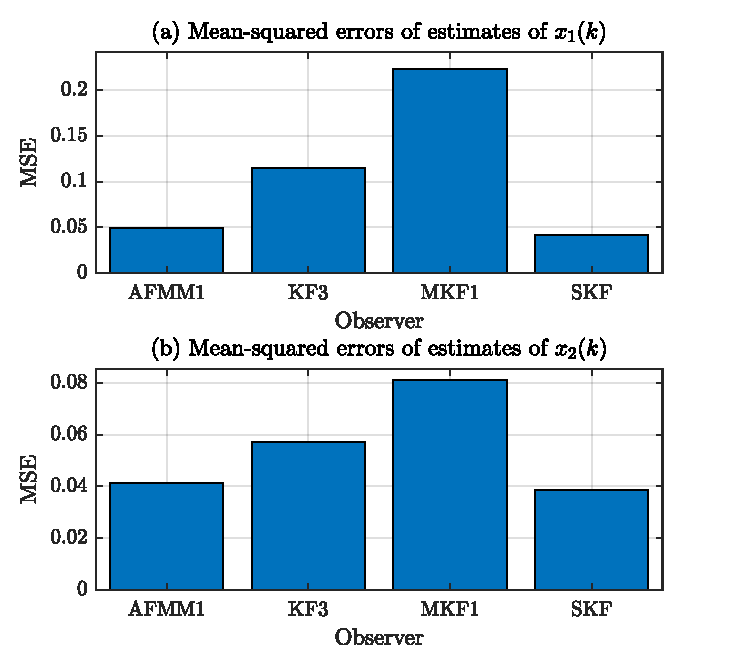
\includegraphics[width=11cm]{images/rod-obs-sim-1-7-MSE-DRAFT.pdf}
	\caption{Comparison of mean-squared errors of observer estimates}
	\label{fig:rod-obs-sim-1-7-MSE}
\end{figure}

\subsection{MIMO linear system OR non-linear system (t.b.d.)}

\begin{figure}[htp]
	\centering
	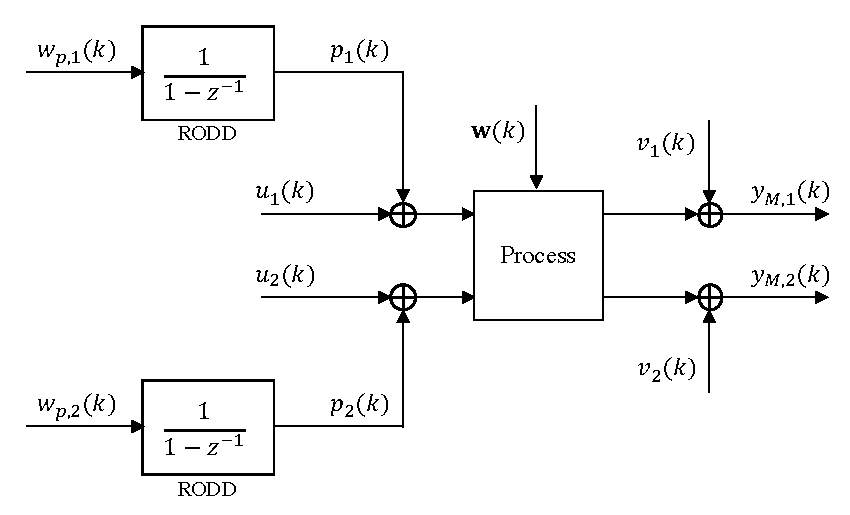
\includegraphics[width=11.5cm]{images/sim-sys-diag-2x2.pdf}
	\caption{Functional diagram of the simulated MIMO system}
	\label{fig:sim-sys-diag-2x2}
\end{figure}

\begin{itemize}
	\item Include similar results using a MIMO system—either the 2x2 linear system or the 0x2 non-linear system used by Robertson et al. (Aromatization process).
	\item Figure \ref{fig:rodd-obs-sim-2-4-ioplot}: input-output data from simulated system
\end{itemize}

\begin{figure}[htp]
	\centering
	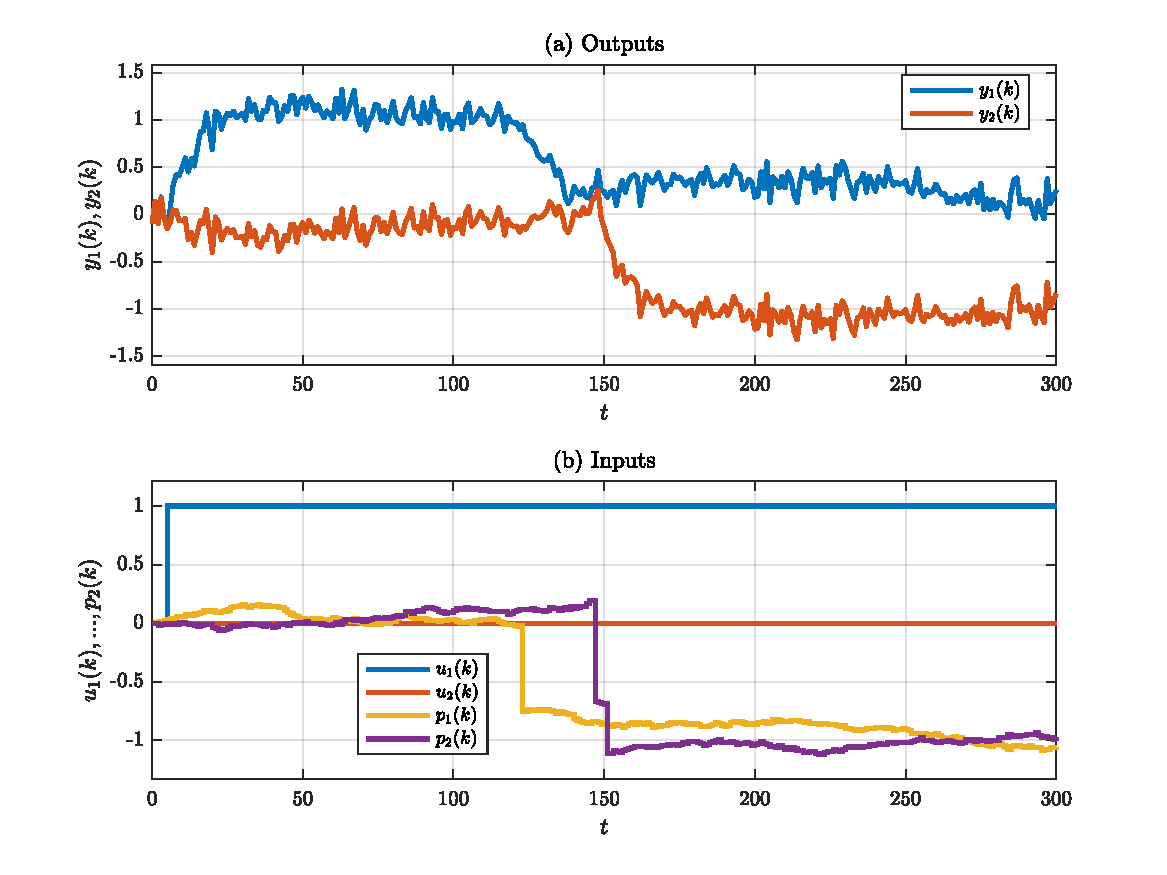
\includegraphics[width=15cm]{images/rod-obs-sim-2-4-ioplot.pdf}
	\caption{Simulation of MIMO linear system with two RODD input disturbances}
	\label{fig:rodd-obs-sim-2-4-ioplot}
\end{figure}

\section{Ore feed disturbance estimation} \label{sim-ore-SISO}

Outline notes:
\begin{outline}
	\1 Unlike previous simulations, this is a non-linear model.
	\1 Describe simulations with grinding simulation model with changing ore properties and changes (same as IFAC paper).
	\1 Describe various data sets generated and their intended use (estimation, validation, statistical performance evaluation).
	\1 Data set used for model identificaiton in Figure: Input-output data – Figure \ref{fig:rod_obs_sim_1_ioplot_P2DcTd4}.
	\1 How process model was identified.
	\1 Augmented model with RODD input step disturbance.
	\1 Use best observer from previous section (sequence pruning).
	\1 Table showing observer paramters.
	\1 Figure: comparison of observer estimates – Figure \ref{fig:rod_obs_sim_1_est_P2DcTd4}.
	\1 Figure: Observer responses to disturbances – Figure \ref{fig:sim_resp_plot}.
	\1 Describe overall performance comparison using metrics in Table \ref{tb:results}.
	\1 Discuss pro's and con's of MMKF observer (steady-state errors vs error in transitions, etc.)
	\1 Discuss applications and potential benefits (e.g. process control, RTO).
	\1 Describe sensitivity analysis simulations.
	\1 Describe sensitivity results:
	\2 (1) to model error, compare Kalman filter and MMKF. Figures \ref{fig:rod_obs_sim_sens_model_KF2_MSE_y_est} and \ref{fig:rod_obs_sim_sens_model_MMKF_MSE_y_est}.
	\2 (2) MMKF sensitivity to RODD model parameters. Figure  \ref{fig:rod_obs_sim_sens_rod_MMKF_MSE_y_est}
\end{outline}

\begin{figure}[htp]
	\centering
	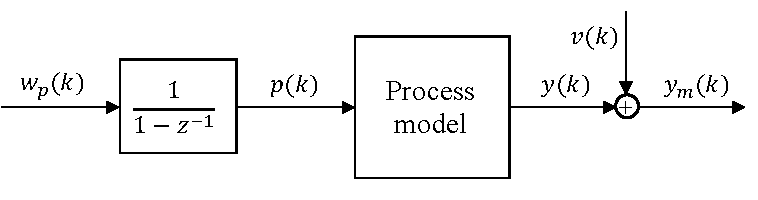
\includegraphics[width=10cm]{images/obs-model-diag.pdf}
	\caption{Observer model structure}
	\label{fig:obs_model}
\end{figure}

\begin{figure}[htp]
	\centering
	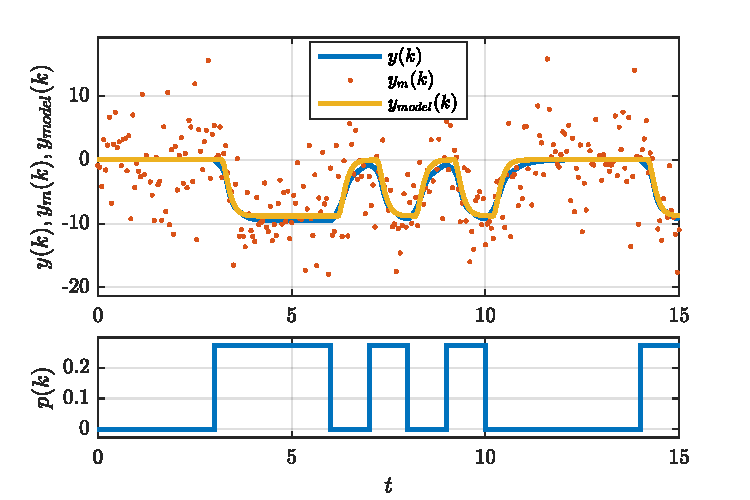
\includegraphics[width=12cm]{images/rod_obs_sim_1_ioplot_P2DcTd4.pdf}
	\caption{Observer model structure}
	\label{fig:rod_obs_sim_1_ioplot_P2DcTd4}
\end{figure}

\begin{figure}[htp]
	\centering
	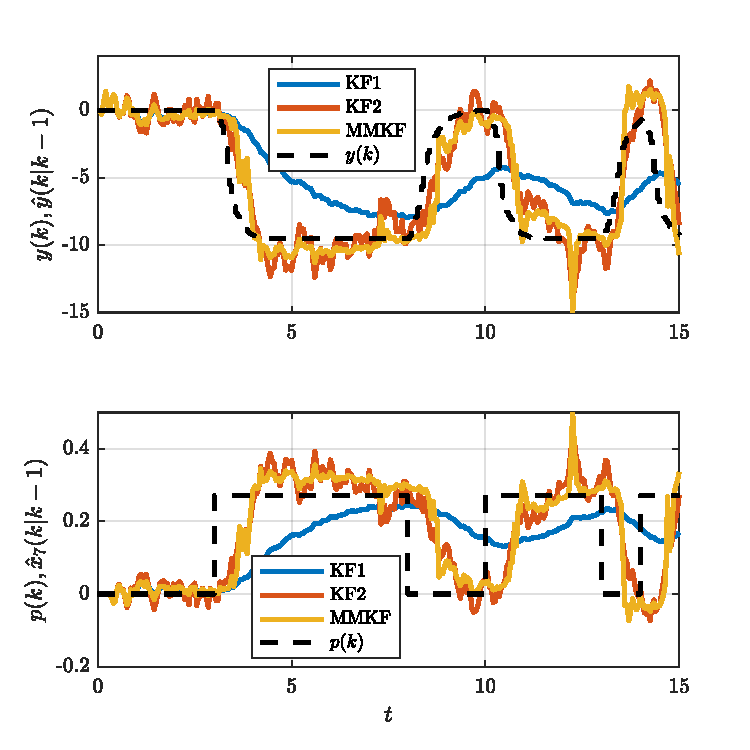
\includegraphics[width=12cm]{images/rod_obs_sim_1_est_P2DcTd4.pdf}
	\caption{Observer estimates}
	\label{fig:rod_obs_sim_1_est_P2DcTd4}
\end{figure}

\begin{figure}[htp]
	\centering
	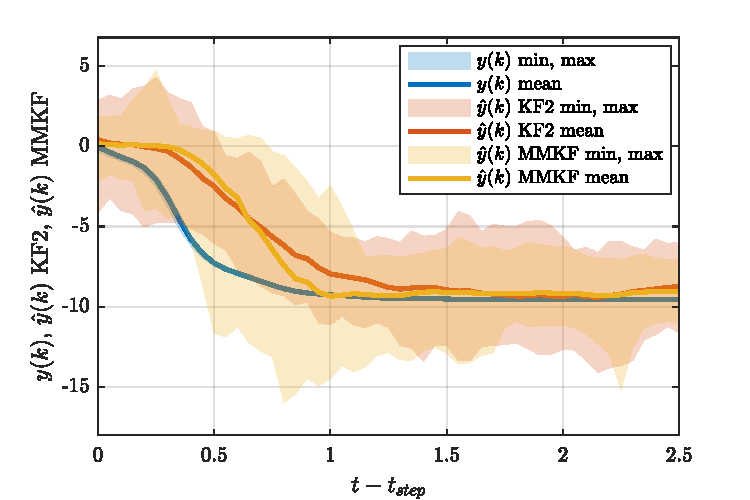
\includegraphics[width=12cm]{images/sim_resp_plot1_P2DcTd4.pdf}
	\caption{Average observer responses to step disturbances}
	\label{fig:sim_resp_plot}
\end{figure}

\begin{table}[hb]
	\begin{center}
		\caption{Observer performance metrics averaged over 50-days of simulation time.} \label{tb:results}
		% See: https://texblog.org/2019/06/03/control-the-width-of-table-columns-tabular-in-latex/
		\begin{tabular}{p{0.34\textwidth}>{\centering\arraybackslash}p{0.08\textwidth}>{\centering\arraybackslash}p{0.08\textwidth}>{\centering\arraybackslash}p{0.08\textwidth}>{\centering\arraybackslash}p{0.08\textwidth}>{\centering\arraybackslash}p{0.08\textwidth}}
			Metric & KF1 & KF2 & KF3 & MMKF & SKF \\
			\hline
			MSE($\hat{y}(k),y(k)$) overall          & 11.0 & 15.9 & 3.7 & 3.5 & 2.1 \\ 
			MSE($\hat{y}(k),y(k)$) transient       & 21.1 & 16.1 & 7.7 & 11.2 & 5.1 \\ 
			MSE($\hat{y}(k),y(k)$) steady-state & 7.9 & 15.9 & 2.5 & 1.1 & 1.1 \\ 
			Var($\hat{y}(k)$) steady-state          & 1.8 & 15.3 & 1.9 & 0.5 & 0.2 \\ 
			MSD($\hat{y}(k),y(k)$) steady-state       & 0.0 & 16.2 & 0.5 & 0.2 & 0.0 \\ 
			% Results for P2DcTd4
			%  Gc = -32.4 * exp(-0.2 * s) / (1 + 0.106*s)^2;
			%                                 KF1       KF3       AFMM        SKF  
			%  MSE                         11.118    3.7395     3.6991     2.0615
			%  MSE in transitions          20.687    7.7201      12.18     5.0674
			%  MSE in steady-state         8.1885     2.521     1.1028     1.1414
			%  Variance in steady-state    1.7723    1.9026    0.39281    0.23769
			%
			% Results for P2Dcd1_T
			%  Gc = -35.94 * exp(-0.05 * s) / ((1 + 0.235*s) * (1 + 0.161*s));
			%                                 KF1       KF3       AFMM        SKF  
			%  MSE                         10.707    3.7702     3.7283     1.9652
			%  MSE in transitions          21.052    7.7605     12.397     4.8145
			%  MSE in steady-state         7.5404    2.5486     1.0745      1.093
			%  Variance in steady-state    1.8111    1.9259    0.39282    0.24514
			
			% Updated results for P2DcTd4 with n_filt = 20, n_min = 18 after fixing
			% initialization between MC simulation runs.
			%  MSE                          11.01    3.6869     3.4952     1.8191
			%  MSE in transitions          21.137    7.7201     11.208     5.0722
			%  MSE in steady-state         7.9091    2.4523     1.1342     0.8232
			%  Variance in steady-state    1.8008    1.9026    0.47604    0.23759
			
			\hline
		\end{tabular}
	\end{center}
\end{table}

\begin{figure}[htp]
	\centering
	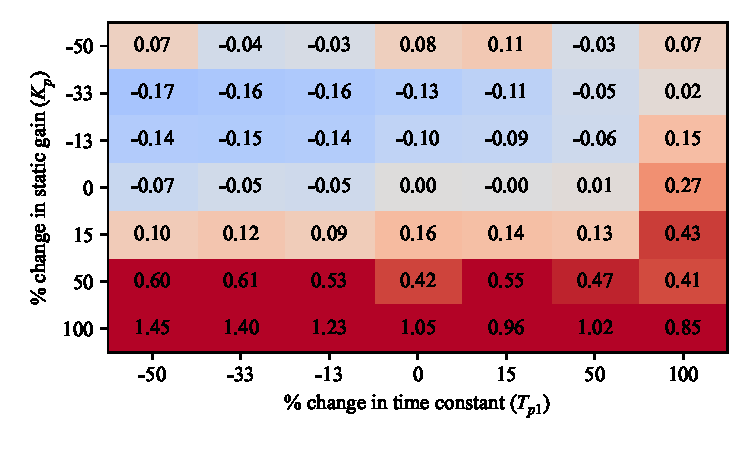
\includegraphics[width=12.5cm]{images/rod_obs_sim_sens_model_KF2_MSE_y_est.pdf}
	\caption{Sensitivity of KF2 estimates to changes in model parameters}
	\label{fig:rod_obs_sim_sens_model_KF2_MSE_y_est}
\end{figure}

\begin{figure}[htp]
	\centering
	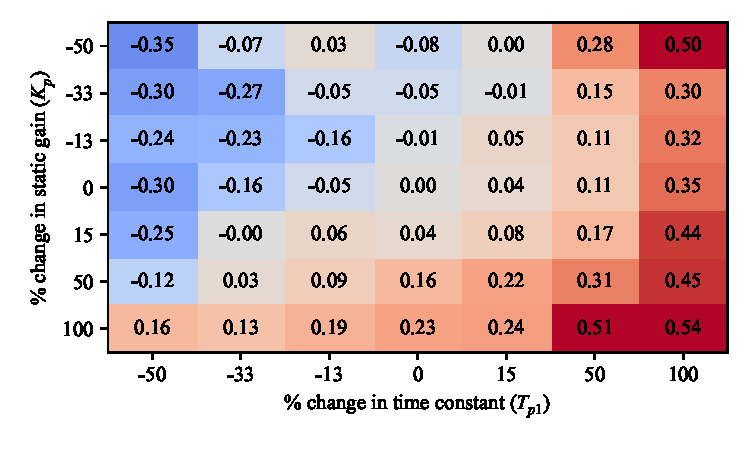
\includegraphics[width=12.5cm]{images/rod_obs_sim_sens_model_MMKF_MSE_y_est.pdf}
	\caption{Sensitivity of MMKF observer estimates to changes in model parameters}
	\label{fig:rod_obs_sim_sens_model_MMKF_MSE_y_est}
\end{figure}

\begin{figure}[htp]
	\centering
	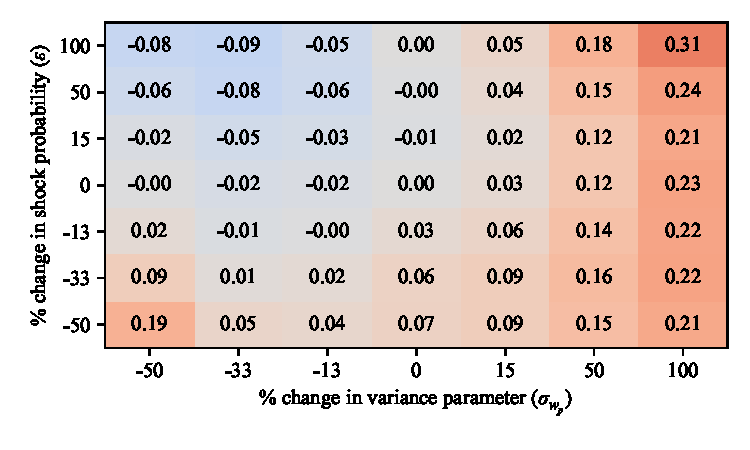
\includegraphics[width=12.5cm]{images/rod_obs_sim_sens_rod_MMKF_MSE_y_est.pdf}
	\caption{Sensitivity of MMKF observer estimates to changes in RODD parameters}
	\label{fig:rod_obs_sim_sens_rod_MMKF_MSE_y_est}
\end{figure}


\section{Grinding circuit control simulation} \label{sim-ore-MIMO} 

Outline notes:
\begin{itemize}
	\item Grinding simulation model in closed loop with MPC controller.
	\item Diagram of feedback system – Figure \ref{fig:sim-mpc-diag}
	\item Table of results - Performance metrics — e.g. tracking error.
	\item Robustness?  E.g. stability margins.
\end{itemize}

\begin{figure}[htp]
	\centering
	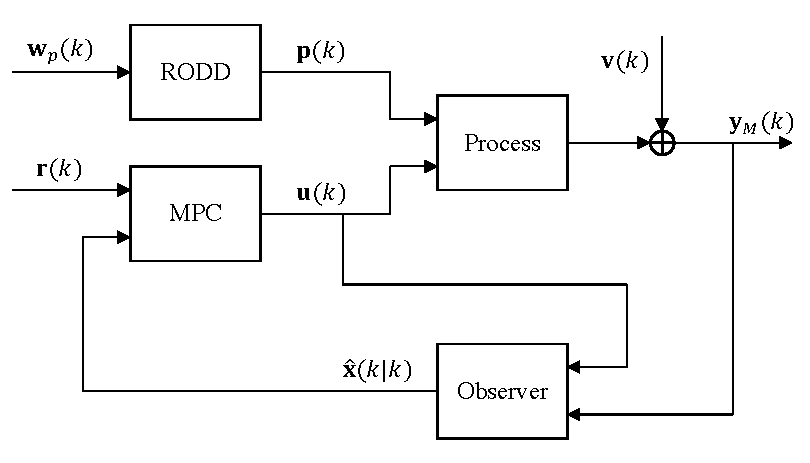
\includegraphics[width=12cm]{images/sim-mpc-diag.pdf}
	\caption{Functional diagram of the simulated feedback control system}
	\label{fig:sim-mpc-diag}
\end{figure}